\documentclass[11pt]{article}
\usepackage{amsmath, amsfonts, amsthm}
\usepackage{graphicx}
\title{CSCI-GA 3033 Assignment 2}
\author{Francis Williams\\N14044150}

\setlength\parindent{0pt}

\begin{document}
\maketitle

\section*{Part 1}
\begin{figure}[ht]
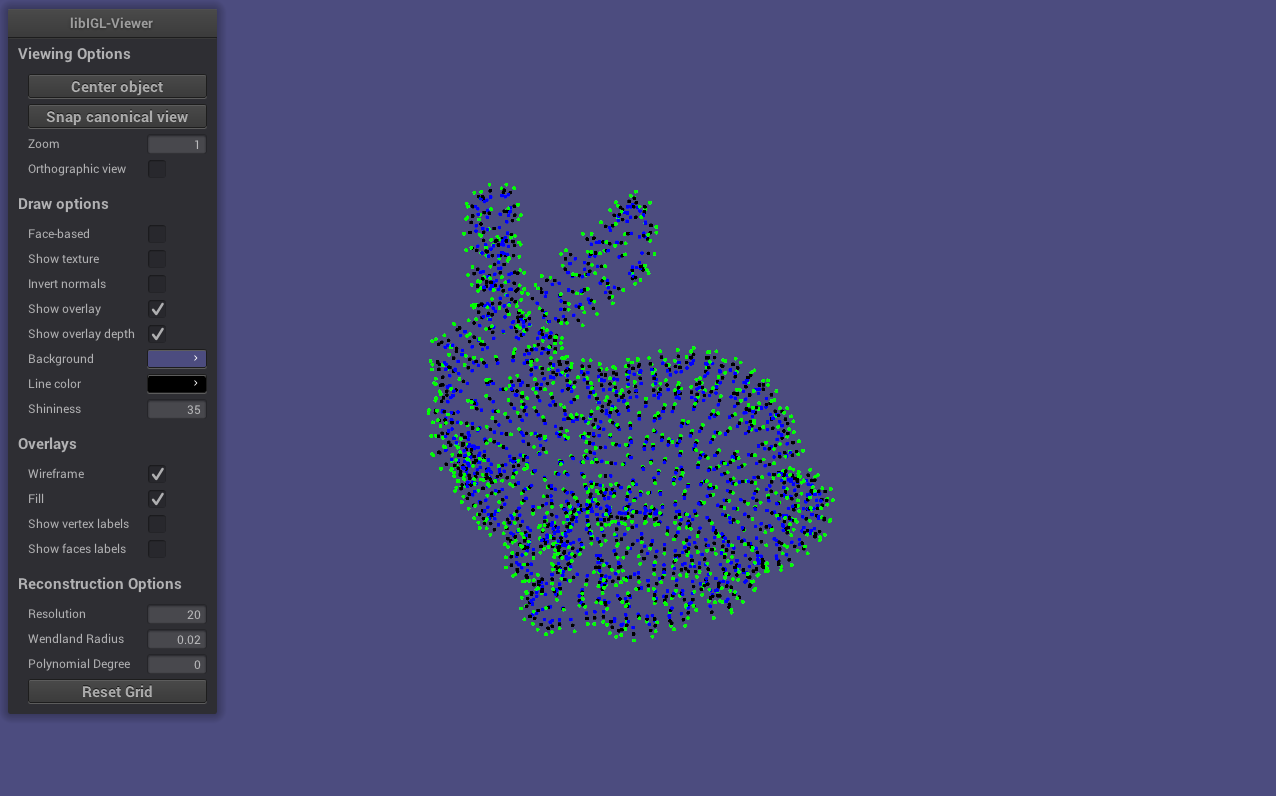
\includegraphics[scale=0.3]{bunny_constraints.png}
\caption{Constraints for the \texttt{bunny-1000.off} model}
\end{figure}

\pagebreak

\section*{Part 2}
\begin{figure}[h]
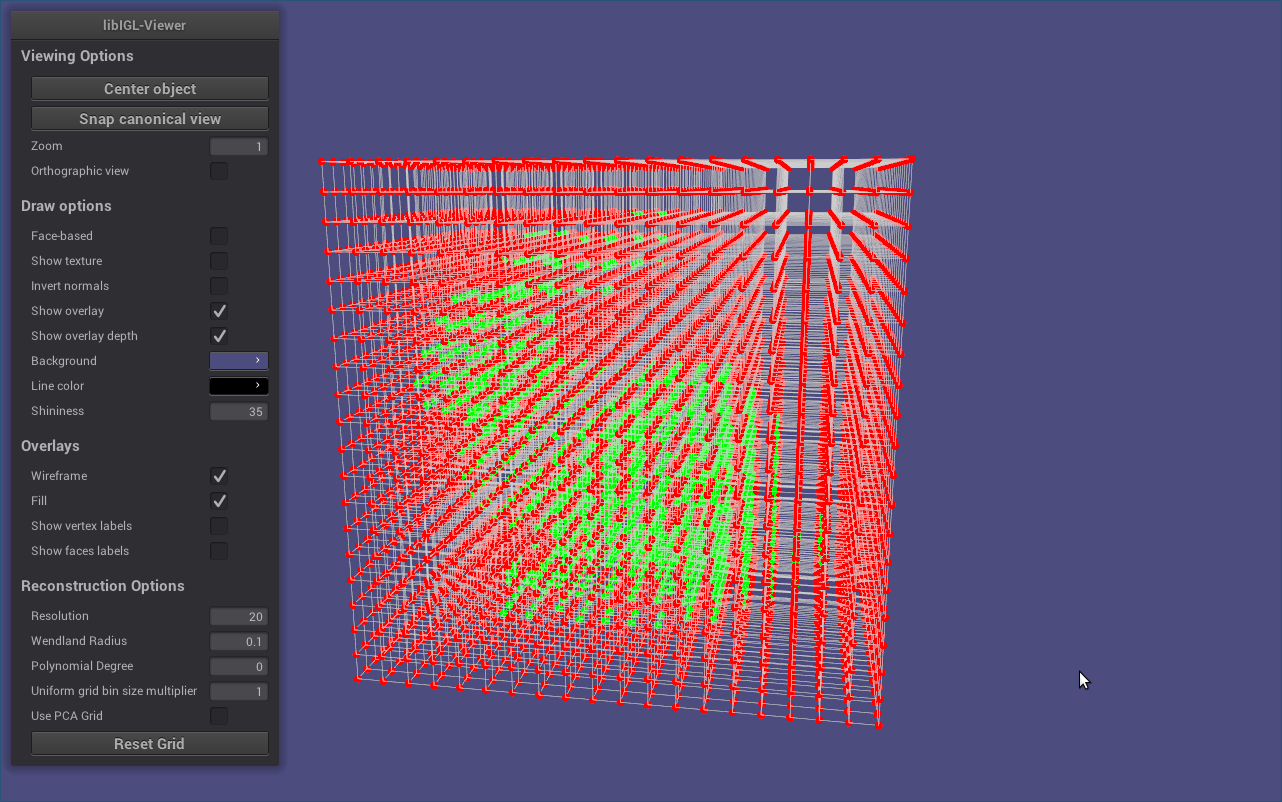
\includegraphics[scale=0.3]{bunny_grid.png}
\caption{Grid values for the \texttt{bunny-1000.off} model}
\end{figure}

\pagebreak

\section*{Part 3}
The reconstructed models can be found in \texttt{data/reconstructed}. The number in the file name refers to one more than the interpolant degree.

\begin{figure}[h]
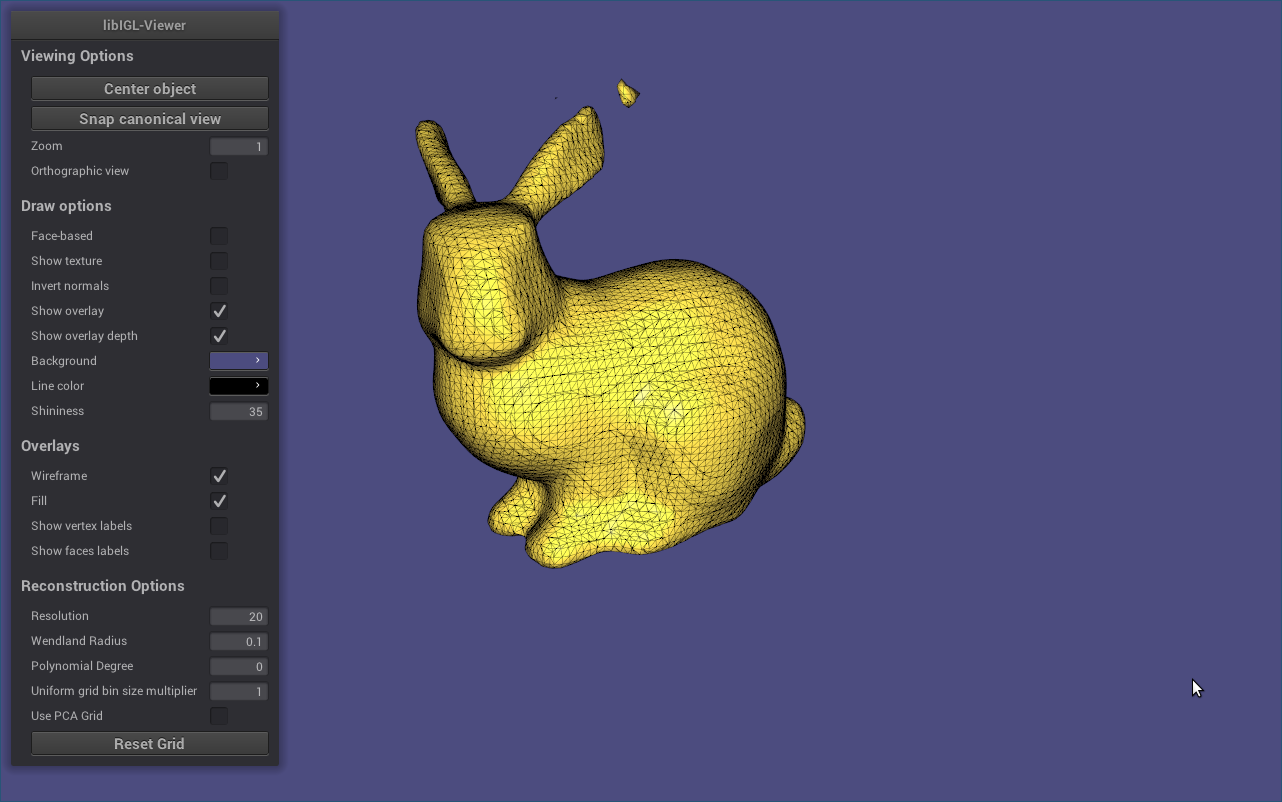
\includegraphics[scale=0.3]{bunny_reconstructed.png}
\caption{Reconstructed \texttt{bunny-1000.off} model}
\end{figure}

\begin{figure}[h]
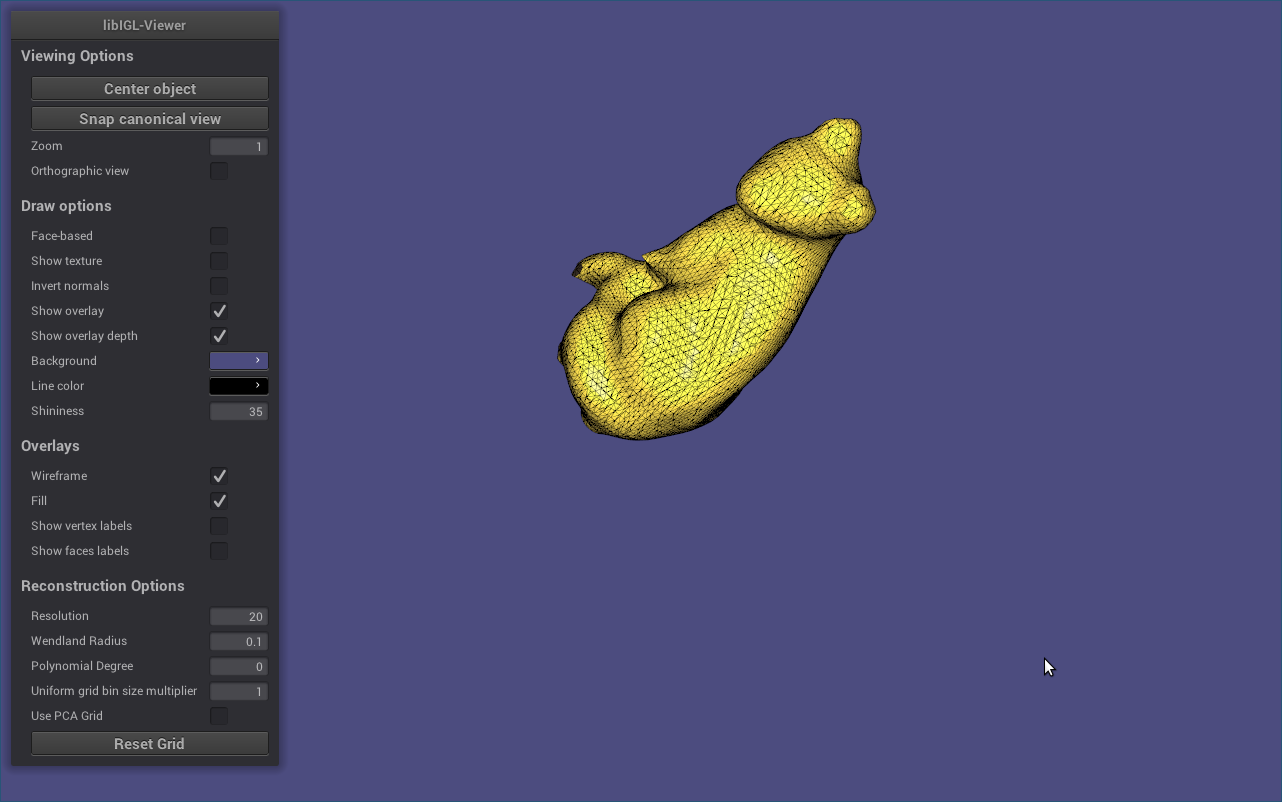
\includegraphics[scale=0.3]{cat_reconstructed.png}
\caption{Reconstructed \texttt{cat.off} model}
\end{figure}

\begin{figure}[h]
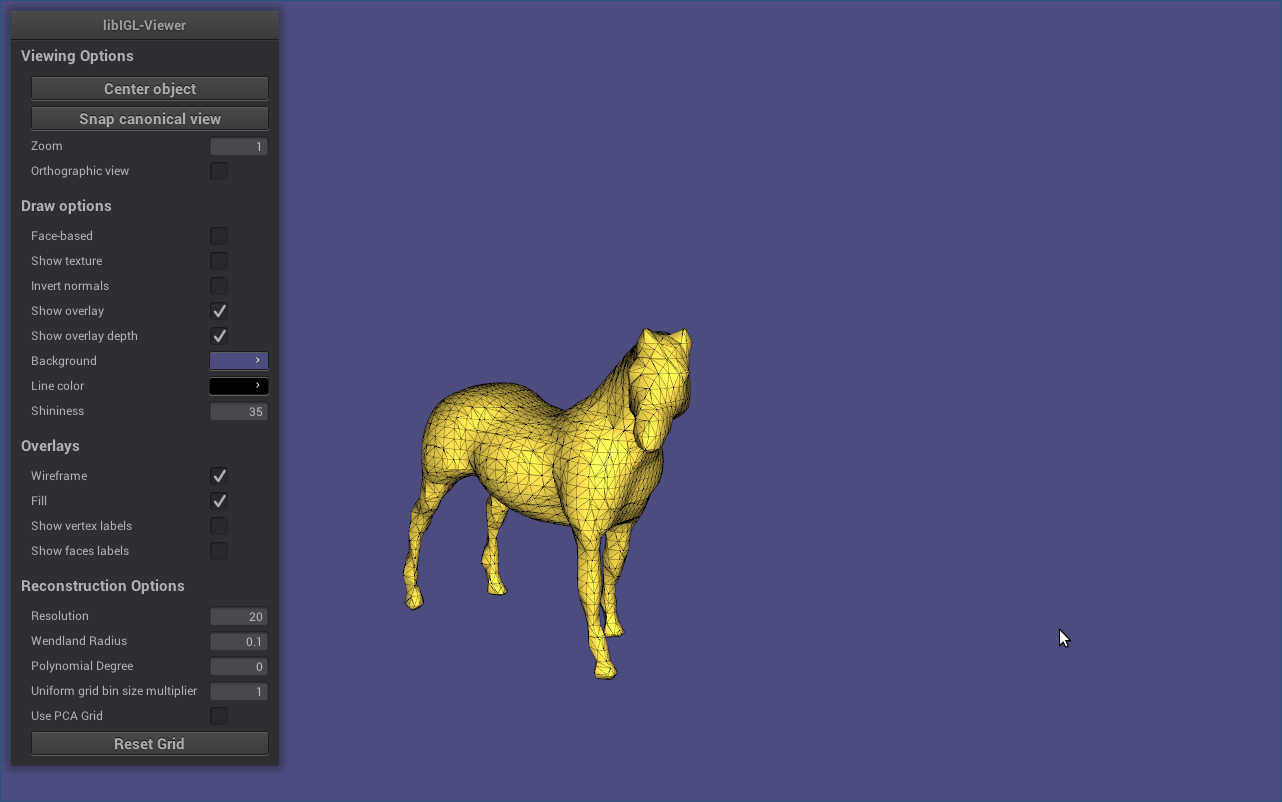
\includegraphics[scale=0.3]{horse_reconstructed.png}
\caption{Reconstructed \texttt{horse.off} model}
\end{figure}

\begin{figure}[h]
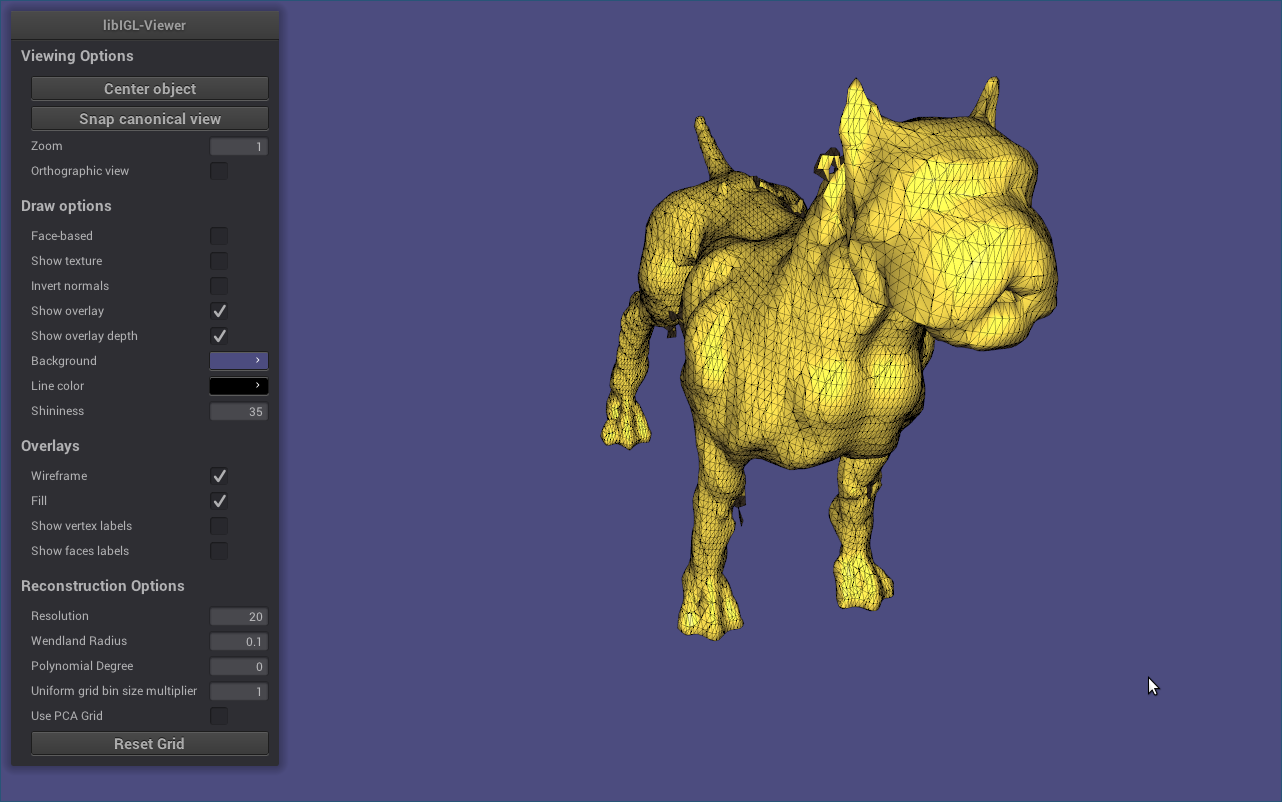
\includegraphics[scale=0.3]{hound_reconstructed.png}
\caption{Reconstructed \texttt{hound.off} model}
\end{figure}

\begin{figure}[h]
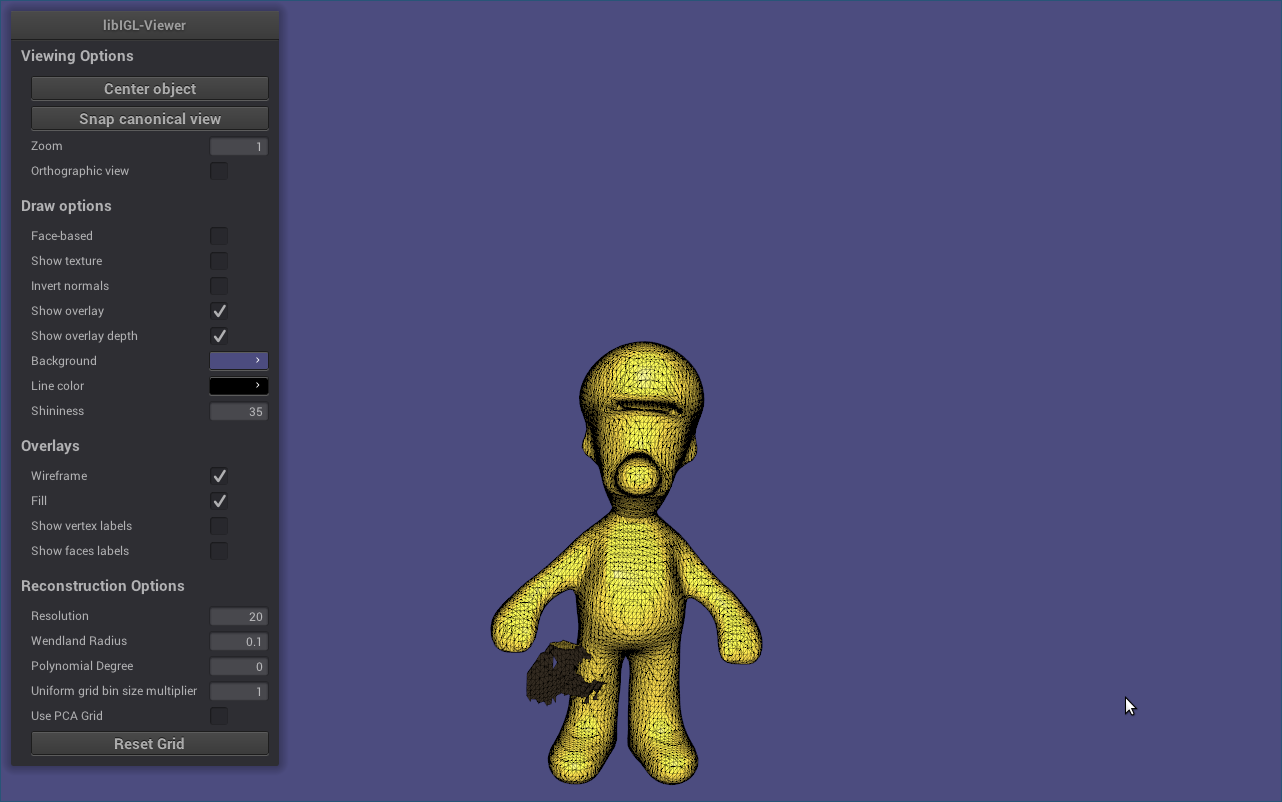
\includegraphics[scale=0.3]{luigi_reconstructed.png}
\caption{Reconstructed \texttt{luigi.off} model}
\end{figure}

\begin{figure}[h]
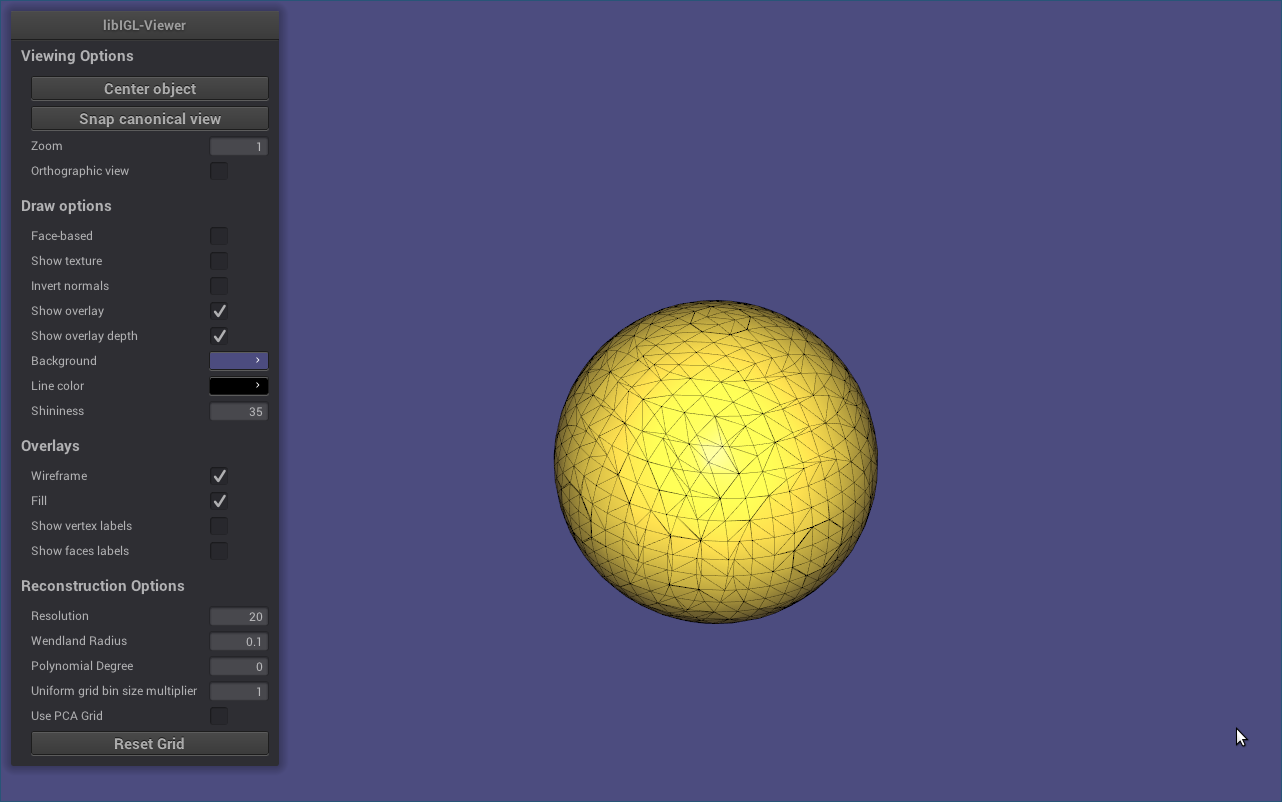
\includegraphics[scale=0.3]{sphere_reconstructed.png}
\caption{Reconstructed \texttt{sphere.off} model}
\end{figure}

\pagebreak

\section*{Theory Question}
\begin{proof}
Let $S$ be the (manifold) implicit surface defined by $f(\mathbf{x}) = 0$, and $p$ be a point on $S$ ($f(p) = 0$). \\

Since we assume $S$ is manifold, there must exist linearly independent vectors $v_1$ and $v_2$ tangent to $S$ at $p$. We can then define the normal as $\bar{n} = v_1 \times v_2$. \\

And since $S$ is the level set of $f$ at $0$, $\nabla_v f = 0$, where $\nabla_v = v \cdot \nabla f$ is the directional derivative along the vector $v$ tangent to $S$. \\

Thefore, $\nabla_{v_1} f = \nabla_{v_2} f = 0 \Leftrightarrow \nabla f \propto v_1 \times v_2 \Leftrightarrow \nabla f \propto \bar{n}$.
\end{proof}

\end{document}
